
\section{Introduction}

This chapter presents the general context of the project.
It introduces the background of the study, formulates the problem statement, explains the proposed solution, and describes the methodological and technical choices adopted throughout the work.

\section{Project Context}

In a world where data is produced continuously by institutions, markets, and digital platforms, decision-makers are increasingly expected to rely on analytical evidence rather than intuition alone.
Economic analysis is one of the domains that benefits the most from this evolution.
Large datasets now make it possible to observe long-term trends, compare periods, detect anomalies, and estimate future dynamics with greater precision.

The housing market is a key component of economic activity.
It is linked to household wealth, bank lending, construction investment, demographic shifts, and public policy.
In the United States, housing prices are especially sensitive to macroeconomic changes.
When interest rates rise, financing conditions become more restrictive.
When unemployment increases, purchasing power and consumer confidence may weaken.
When inflation accelerates, the overall cost environment changes, which can also affect real estate dynamics.

Traditional approaches remain useful for descriptive interpretation, but they may fail to capture more complex interactions between variables.
This is why data mining and machine learning are particularly relevant in this context.

\subsection{Academic Context}

This work was developed as part of a tutored project in Data Mining and Machine Learning.
The aim of the course is to move from theory to practice by applying modern analytical methods to a realistic case study.
The project therefore combines academic concepts with implementation choices that reflect practical data science work.

\section{Project Presentation}

\subsection{Problem Statement}

The central research question of this project can be stated as follows:

\begin{quote}
How can data mining and machine learning techniques be used to analyze and predict housing market trends in the United States based on macroeconomic indicators?
\end{quote}

This question involves several sub-problems:
\begin{itemize}
\item identifying which variables are the most informative,
\item preprocessing heterogeneous data into a usable format,
\item selecting appropriate machine learning models,
\item evaluating predictive performance,
\item and presenting the results in an accessible interface.
\end{itemize}

\subsection{Critique of Existing Approaches}

A review of common approaches shows that many economic analyses rely either on simple descriptive statistics or on highly specialized econometric models.
Descriptive methods are easy to understand but not sufficient for prediction.
Econometric approaches are rigorous but can become difficult to deploy in an accessible application.
In contrast, machine learning offers flexible tools that can learn from data directly, especially when relationships are non-linear or when multiple indicators must be analyzed jointly.

Still, machine learning also has limitations.
Some models may be difficult to interpret, and performance depends strongly on data quality.
This project therefore adopts a balanced approach that combines interpretable and more powerful models.

\subsection{Proposed Solution}

The proposed solution is based on three major components:
\begin{enumerate}
\item a data analysis workflow for understanding the dataset,
\item predictive models for estimating housing trends,
\item and an interactive dashboard for visualization and decision support.
\end{enumerate}

The analysis begins with data preprocessing and exploratory data analysis.
Next, machine learning models are trained and evaluated.
Finally, the results are integrated into a Streamlit dashboard to provide an interactive user experience.

\section{Methodological Study}

\subsection{Classical and Agile Methods}

Classical project methods generally follow a sequential logic.
They are useful when the scope is stable from the beginning.
However, data science projects often evolve as the analyst discovers data limitations, new variables, or improved modeling strategies.
For this reason, a more iterative logic is needed.

Agile methods promote flexibility and frequent adjustment.
Although this project is academic rather than industrial, it benefits from an iterative mindset.
Several parts of the work, especially feature selection and dashboard design, were refined progressively.

\subsection{Why CRISP-DM}

The methodology selected for this project is CRISP-DM, which stands for Cross-Industry Standard Process for Data Mining.
It is one of the most widely used methodologies in analytical projects because it provides a clear structure while remaining adaptable.

The six CRISP-DM phases are:
\begin{enumerate}
\item Business Understanding
\item Data Understanding
\item Data Preparation
\item Modeling
\item Evaluation
\item Deployment
\end{enumerate}

\subsubsection{Business Understanding}
This phase defines the objective of the project and clarifies why the problem matters.
In our case, the business objective is to better understand housing market dynamics and build a useful predictive tool.

\subsubsection{Data Understanding}
This phase focuses on exploring the available variables, checking their types, identifying anomalies, and inspecting their overall quality.

\subsubsection{Data Preparation}
This phase includes cleaning, date parsing, missing value handling, scaling, and feature engineering.
It is a critical phase because the quality of the models depends strongly on the quality of the prepared dataset.

\subsubsection{Modeling}
In this project, Ridge Regression and Random Forest were selected as the main predictive models.
They represent two complementary perspectives: interpretability and predictive power.

\subsubsection{Evaluation}
Evaluation makes it possible to compare models objectively.
Metrics such as MAE, RMSE, and \(R^2\) are used to judge performance.

\subsubsection{Deployment}
The final step is deployment through a Streamlit dashboard.
This transforms the project from a technical notebook into a usable analytical application.

\section{Technologies and Development Environment}

Python was selected as the main language because it offers a rich ecosystem for data science.
The following tools were used throughout the project:
\begin{itemize}
\item \textbf{Pandas} for tabular data manipulation,
\item \textbf{NumPy} for numerical operations,
\item \textbf{Scikit-learn} for preprocessing, modeling, and evaluation,
\item \textbf{Plotly} for interactive visualization,
\item \textbf{Streamlit} for dashboard development.
\end{itemize}

The development process was carried out using common tools such as Jupyter Notebook and Visual Studio Code.
These environments supported experimentation, testing, and iterative refinement.

\section{Project Planning}

The work was structured into several phases:
\begin{itemize}
\item data collection and understanding,
\item preprocessing and exploratory analysis,
\item model development and testing,
\item dashboard implementation,
\item result interpretation and report writing.



\end{itemize}

\begin{figure}[H]
\centering
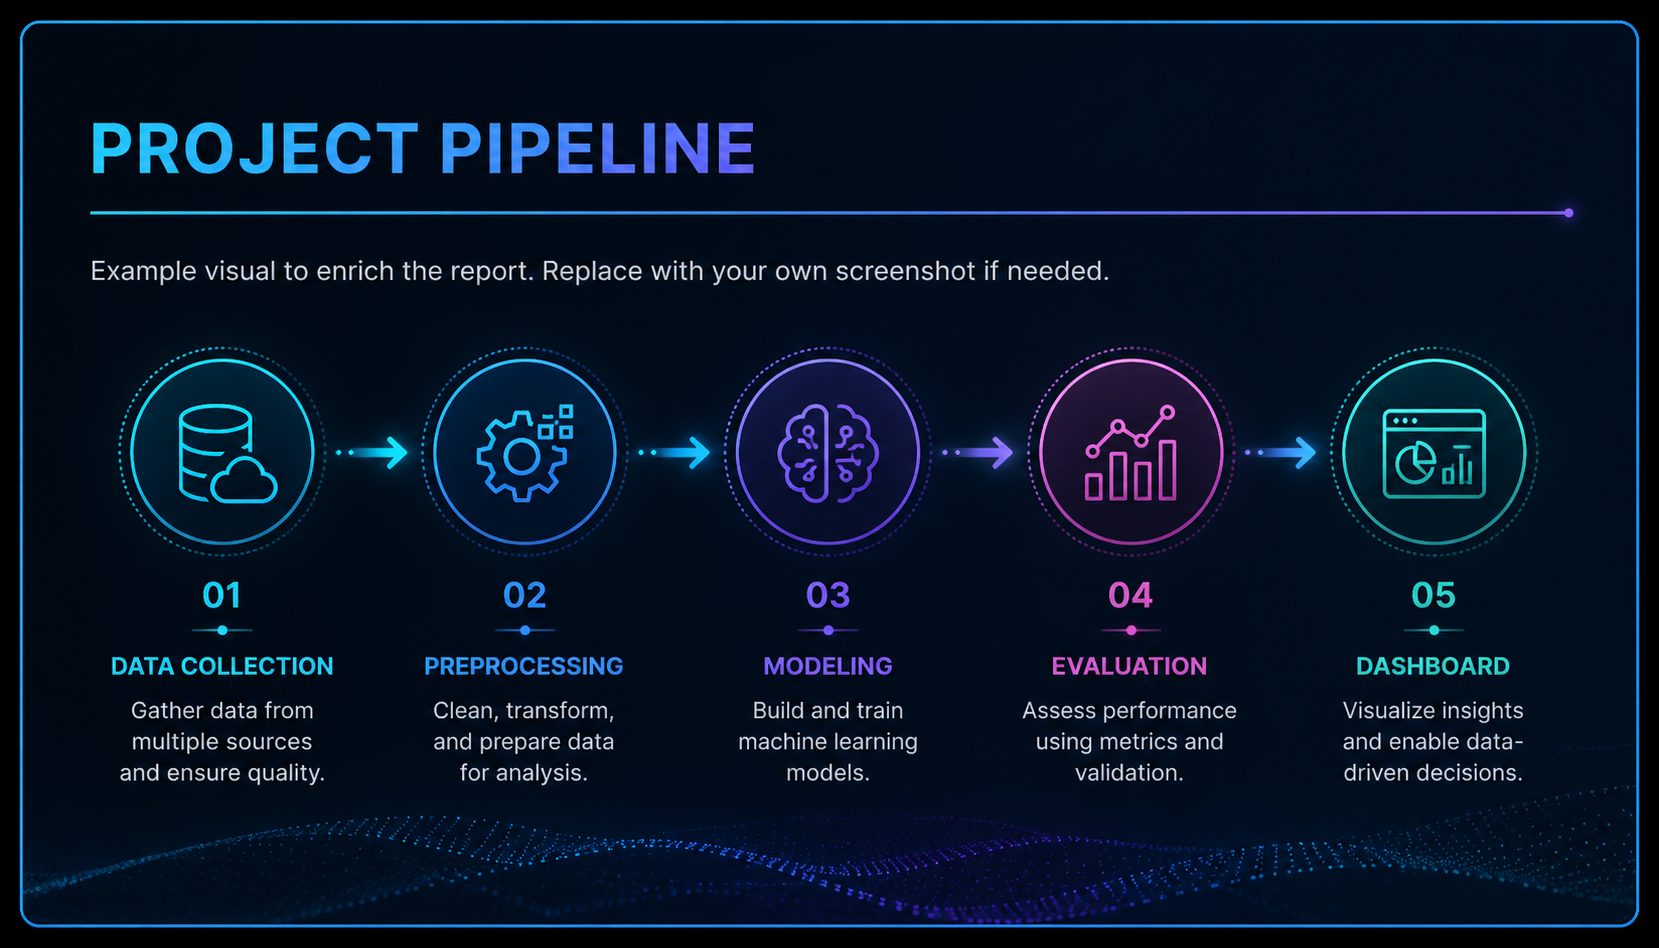
\includegraphics[width=0.85\textwidth]{project_pipeline (2).png}
\caption{Illustrative pipeline of the project workflow.}
\label{fig:pipeline}
\end{figure}

The planning followed an incremental logic.
Early work focused on understanding the data.
Later work concentrated on model comparison and dashboard enhancement.
This progression allowed the project to remain aligned with its objectives while adapting to practical findings.
\section*{Gantt Chart }

\begin{center}
\begin{ganttchart}[
    time slot format=isodate,
    compress calendar,
    x unit=0.7cm,
    y unit chart=0.9cm,
    bar height=0.6,
    vgrid, hgrid,
    bar label font=\small\rmfamily,
    group label font=\bfseries\small,
    title label font=\bfseries\small,
    title/.style={draw=none, fill=none},
    label text width=4cm,
    label text font=\small,
    expand chart=\textwidth
]{2025-02-01}{2025-05-17}

\gantttitlecalendar{month=name}\\

\ganttbar{Problem Analysis}{2025-02-01}{2025-02-10} \\
\ganttbar{Report Writing}{2025-02-11}{2025-02-15} \\
\ganttbar{Requirement Analysis}{2025-02-16}{2025-02-29} \\
\ganttbar{Report Writing}{2025-03-01}{2025-03-05} \\
\ganttbar{System Design}{2025-03-06}{2025-03-20} \\
\ganttbar{Report Writing}{2025-03-21}{2025-03-25} \\
\ganttbar{Implementation}{2025-03-26}{2025-04-15} \\
\ganttbar{Report Writing}{2025-04-16}{2025-04-20} \\
\ganttbar{Testing \& Debugging}{2025-04-21}{2025-05-10} \\
\ganttbar{Report Writing}{2025-05-11}{2025-05-17} \\
\end{ganttchart}

\vspace{0.5em}
\textbf{Figure: Project Timeline }
\end{center}



\begin{table}[H]
\vspace*{\fill}
\centering
\Large
\renewcommand{\arraystretch}{2.0} % increase row height

\caption{Project Schedule}

\begin{tabular}{|p{6cm}|c|c|c|}
\hline
\textbf{Task Name} & \textbf{Start Date} & \textbf{End Date} & \textbf{Duration (days)} \\
\hline
Problem Analysis           & 01-Feb-2025 & 10-Feb-2025 & 10 \\
Report Writing             & 11-Feb-2025 & 15-Feb-2025 & 5  \\
Requirement Analysis       & 16-Feb-2025 & 29-Feb-2025 & 14 \\
Report Writing             & 01-Mar-2025 & 05-Mar-2025 & 5  \\
System Design              & 06-Mar-2025 & 20-Mar-2025 & 15 \\
Report Writing             & 21-Mar-2025 & 25-Mar-2025 & 5  \\
Implementation             & 26-Mar-2025 & 15-Apr-2025 & 21 \\
Report Writing             & 16-Apr-2025 & 20-Apr-2025 & 5  \\
Testing \& Debugging       & 21-Apr-2025 & 10-May-2025 & 20 \\
Report Writing             & 11-May-2025 & 17-May-2025 & 7  \\
\hline
\end{tabular}

\vspace*{\fill}
\end{table}



\section{Analytical Scope of the Project}

The project is built around a clear objective: analyzing the relationship between the United States housing market and macroeconomic indicators while creating a Streamlit dashboard to visualize, compare, predict, and interpret housing-price behavior. This objective is implemented through a complete housing intelligence platform.

The platform includes the following functional blocks:
\begin{itemize}
\item \textbf{OLAP analysis}: multidimensional exploration through pivot tables, grouped metrics, and segmentation.
\item \textbf{AI chatbot}: natural language interaction with the project and its results.
\item \textbf{Prompt chatbot}: structured prompt-based guidance for users who want analytical explanations without coding.
\item \textbf{Unsupervised learning}: K-Means, DBSCAN, PCA, and anomaly detection to discover hidden patterns.
\item \textbf{Reinforcement learning}: an educational decision-policy module that illustrates state, action, reward, and policy logic.
\item \textbf{Paper review and comparison}: comparison between project findings, economic theory, and market-period interpretation.
\item \textbf{Streamlit deployment}: a complete interactive product with navigation, styling, export, and production-readiness checks.
\item \textbf{Model governance}: experiment tracking, model registry, validation checks, and model-card style interpretation.
\end{itemize}

This scope is important because real data science projects rarely stop at a single model. A useful analytical product must also provide interpretation, reproducibility, usability, and decision support. The extended project therefore moves closer to a professional workflow used in companies, banks, consultancies, and public institutions.

\section{Business Value}

The dashboard can support several types of users:
\begin{itemize}
\item \textbf{Students and researchers} can use the platform to understand how machine learning models behave on economic data.
\item \textbf{Real estate analysts} can explore market indicators, compare periods, and interpret housing-price movement.
\item \textbf{Financial institutions} can use the workflow as a prototype for risk monitoring, scenario analysis, and affordability analysis.
\item \textbf{Policy-oriented users} can compare macroeconomic periods and study how housing indicators evolved under different market conditions.
\end{itemize}

The value of the project is therefore not only technical. It is also educational and managerial. It helps transform raw economic data into understandable insight.

\section{CRISP-DM Mapping}

The project still follows CRISP-DM, but each phase now contains additional components.

\begin{longtable}{p{4cm}p{11cm}}
\toprule
\textbf{CRISP-DM phase} & \textbf{Implementation in the project} \\
\midrule
Business Understanding & Definition of the housing market problem, business impact, user needs, and decision-support objectives. \\
Data Understanding & Dataset preview, date detection, numeric profiling, missing-value checks, duplicate checks, and correlation exploration. \\
Data Preparation & Column cleaning, date parsing, numeric conversion, administration labeling, lag features, rolling means, differencing, and imputation. \\
Modeling & Regression, classification, model comparison, forecasting, clustering, PCA, anomaly detection, and reinforcement-learning simulation. \\
Evaluation & MAE, RMSE, R squared, accuracy, precision, recall, F1-score, ROC AUC, clustering quality metrics, and interpretability checks. \\
Deployment & Streamlit dashboard, export modules, AI chatbot, prompt interaction, production-readiness checks, experiment tracking, and model registry. \\
\bottomrule
\caption{Mapping between CRISP-DM and the analytical platform.}
\end{longtable}

\section{Functional Requirements}

The system must satisfy the following functional requirements:
\begin{enumerate}
\item Load a housing and macroeconomic dataset from a default path or user upload.
\item Clean and prepare the dataset automatically.
\item Detect the date column and generate time-based comparisons.
\item Visualize trends, correlations, distributions, and administration-level differences.
\item Train supervised models for regression and classification tasks.
\item Compare several models using standard evaluation metrics.
\item Generate forecasts using lagged and rolling variables.
\item Apply unsupervised learning to discover clusters and anomalies.
\item Provide OLAP-style pivot and segmentation analysis.
\item Offer chatbot and prompt-based assistance for interpretation.
\item Export reports, tables, and insights.
\item Present production-readiness and governance checks.
\end{enumerate}

\section{Non-Functional Requirements}

The platform must also satisfy non-functional requirements:
\begin{itemize}
\item \textbf{Usability}: the dashboard must be understandable to non-technical users.
\item \textbf{Modularity}: the code should be organized into reusable helper functions.
\item \textbf{Reproducibility}: data cleaning, model training, and evaluation steps must be documented.
\item \textbf{Interpretability}: the system should explain why a model or variable is important.
\item \textbf{Scalability}: the design should allow future modules or datasets to be added.
\item \textbf{Reliability}: validation checks should warn the user before trusting weak data or unstable models.
\end{itemize}

\section{Project Contribution}

The project contributes a broad and realistic data science workflow. The contribution can be summarized in four points:
\begin{enumerate}
\item It connects housing-market analysis with macroeconomic interpretation.
\item It combines classical supervised learning with unsupervised learning and reinforcement-learning concepts.
\item It adds an interaction layer through AI and prompt-based assistance.
\item It introduces production-readiness ideas that are often missing in academic dashboards.
\end{enumerate}

This makes the project stronger academically because it demonstrates both technical skills and methodological understanding.

\section{Conclusion}

This chapter introduced the context, problem, objectives, methodology, and technologies of the project. It established the general framework of the study and justified the use of data mining, machine learning, OLAP analysis, AI-assisted interpretation, and interactive deployment for housing market analysis. The chapter also clarified the functional and non-functional requirements that guide the platform design. The next chapter presents the theoretical background required to understand the selected methods in greater detail.
